\chapter{データセット}
\label{chap:dataset}
\fancyhf{}
\rhead{\thepage}
\lhead{第\ref{chap:dataset}章 データセット}
\cfoot{\thepage}


本章では,実験で用いるデータセットについて述べる.

本研究では,
オンライン学習サイトにおける,生徒の問題回答ログをデータとして用いる.

その際,比較検証のため,
教科を数学に絞った上で,2つのデータセットを用意する.
いずれのデータセットも,前章で述べたデータセットの要件の一つである,既存の知識タグを有するという要件を満たしている.

以下では,各データセットについて概説した後,
本研究に適用するためのデータの抽出方法について述べる.


\section{ASSISTments 2009-2010}
本データセットは,オンライン学習サービスの「ASSISTments\footnote{\url{https://www.assIstments.org/}}」
における,生徒の問題回答ログから生成されている.
まず,ASSISTmentsのサービスについて概説した後,
本研究で用いるデータセットについて説明する.
その際,本研究に適用する際に問題となるデータの性質に言及した上で,
その問題点を解消するためのデータの抽出方法を述べる.

\subsection{ASSISTmentsのサービス}
ASSISTmentsはIntelligent Tutoring System(ITS)の一つで,
2017年1月現在で,14の国と42の州において利用されている.
数学や科学,英語や社会と言った科目をカバーしており,レベルは日本における小学生から高校生まで様々である.
基本的な仕組みは,システムが生徒に課した問題を生徒が回答し,その結果をシステムが自動的に採点,間違えた場合はヒントを出すなどして,生徒の知識獲得を促すもので,
教師や親がその回答結果や統計情報かた生徒の習熟度を確認できること,
また,必要があれば,システム上で提供されている教材を自由に編集して,新たな問題を作成できる柔軟性の高さなどから,
様々な教育機関や,オンライン教育サービス上で活用されている.


\subsection{対象データセット}
本研究で用いるデータセットは,「ASSISTments 2009-2010」と呼ばれる,
ASSISTmentsにおける,生徒の2009年から2010年の間の数学の問題回答ログの内,
「skill\_builder」\footnote{\url{https://sites.google.com/site/assistmentsdata/home/assistment-2009-2010-data/skill-builder-data-2009-2010}}
と呼ばれるデータセットである.

元々,「ASSISTments 2009-2010」には
「skill\_builder」と「non\_skill\_builder」という,
系統の異なる2つのデータセットが含まれている.
「skill\_builder」は,生徒に知識を段階的に身につかせることを目的にした系統で,
ある知識を問う問題に生徒が連続で正答できた場合に,該当の知識を習得したものとみなし,次に進ませるというものである.
日本の教育現場で言えば,授業ごとの小テストに近いものといえる.
一方,「non\_skill\_builder」は,生徒がそれまで学んできたことを正しく身につけられているかを確認することを目的にした系統で,
さまざまな知識を問う問題を,まとめて生徒に課すものである.
日本の教育現場で言えば,期末テストに近いものといえる.

このような性質から,「skill\_builder」のデータセットの方が,生徒の知識獲得過程の細かな推移を観察する上で適しているため,
Deep Knowledge Tracing\cite{piech2015deep}を始めとする,Knowledge Tracingに関する多くの研究で利用されるデータセットであり,
本研究でも同様に,「skill\_builder」のデータセットを用いる.
% 概観
生徒が解く問題(problem)には,1つ以上の知識タグ(skill)が紐付いている.
「skill\_builder」のデータセットには,4,217人の生徒の,124の知識タグが紐づく26,688の問題に対する,401,756の回答ログが含まれている.
なお,「skill\_builder」のデータセットは,行の重複などによって大幅な不備が指摘されたため訂正版が提供されており,
それ以前の研究結果は信憑性が低い.本研究では,訂正後のデータセットを用いている.


\subsection{データの抽出}
%抽出条件
本データセットは,本研究に適用する上で以下の3つの問題を抱えている.順に,各問題と対策について述べる.

まず,問題(problem)の中には複数の知識タグ(skill)が紐付いているものがあるが,そうした問題が回答された場合には,
知識タグの数だけ,ログが別々に作成されている.
これは,見かけ上のログ数(401,756)が,実際に回答された回数より多くなっているだけでなく,
同時に回答された問題や知識タグが,別々に回答されたとみなされる危険性があり,
この前提を考慮しないKnowledge Tracingは不適切であることが指摘されている\cite{xiong2016going}.
このため,重複している行を一つにまとめる作業が必要である.

次に,既存の知識タグ(skill)についても,存在はするものの,名前が割り当てられていないものが存在し,
これらは抽出された知識タグと比較することが不可能なため,除外する必要がある.


また,本データセットは,全体で見ると十分大規模であるといえるが,
個別の問題に関して言えば,ほとんど回答されていない問題が,
全体に対して大きな割合を占めている.(図\ref{fig:assistmets}を参照)
十分なログ数を保有しない問題は,大規模データから深層学習によって知識タグを抽出するという本研究の目的を満たさないため,
ログ数について一定の閾値を設けてデータセットを切り分けることによって,適切なデータを抽出する必要がある.


以上より,本研究では,元のデータセットから,以下の方法で分析対象とするデータを抽出している.
1)同時回答を意味する重複行を一つにまとめる.
2)名前が割り当てられている知識タグを持つ問題に関するログのみを抽出する.
3)2)のうち,最低30回以上回答されている問題に関するログのみを抽出する.
4)3)に含まれる問題を,最低2回以上回答している生徒に関するログを抽出する.

なお,3)の30回以上という具体的な数字は,深層学習として有意な結果が得られるログ数として,実験的に得たものであり,網羅的に検証されたものではない.
4)の2回以上という数字は,知識獲得の推移を観察する上で最低限必要なログ数である.
%結果的に,2,809人の,31の知識タグが紐づく967の問題に対する,66,707の回答ログが分析対象である.
結果的に,3,410人の,56の知識タグが紐づく2,635の問題に対する,129,317の回答ログが分析対象である.

\begin{figure}[t]
\begin{center}
\hspace*{-40pt}\makebox[1.2\textwidth][c]{
	\minipage{0.53\textwidth}
		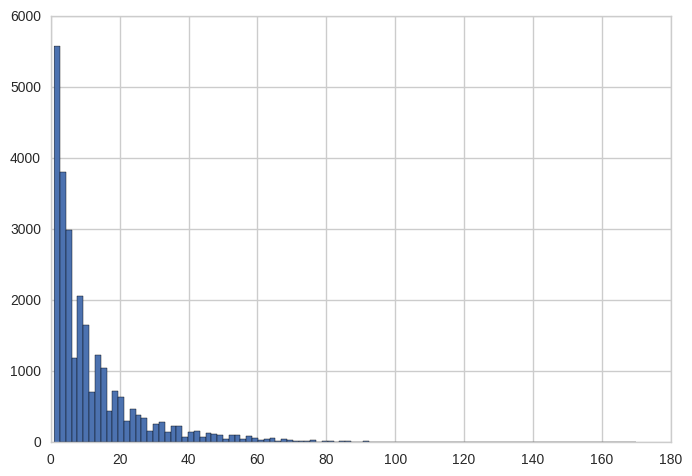
\includegraphics[width=180pt]{./img/assistments_problem_dist.png}
		\caption{「ASSISTments 2009-2010」における問題ごとの回答数の分布}
		\label{fig:assistments}
	\endminipage\hfill
	\minipage{0.53\textwidth}
		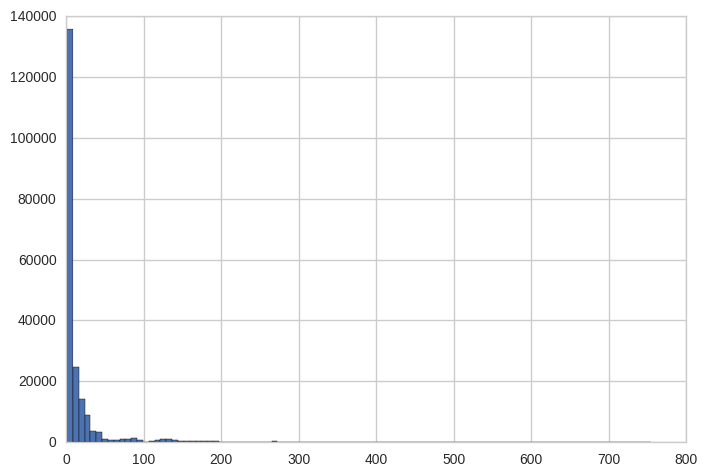
\includegraphics[width=180pt]{./img/kdd_problem_dist.png}
		\caption{「bridge to algebra 2006-2007」における問題ごとの回答数の分布}
		\label{fig:kdd}
	\endminipage\hfill
}
\end{center}
\end{figure}


\section{bridge to algebra 2006-2007}
本データセットが利用された「KDDCup」について概説した後,
データセット自体について説明する.
その際,ASSISTments同様,本研究に適用する際に問題となるデータの性質に言及した上で,
その問題点を解消するためのデータの抽出方法を述べる.


\subsection{KDDCup}
「KDDCup(Knowledge Discovery and Data Mining Cup)\footnote{\url{http://www.kdd.org/kdd-cup}}」は、
100以上の国にまたがり、10万人を超える会員を持つコンピューターサイエンス分野の学会である「ACM(the Association for Computing Machinery)」の分科会である
「SIGKDD(Special Interest Group on Knowledge Discovery and Data Mining)」が毎年開催する競技会であり、
この分野で最も古く権威のある競技会の一つである.


\subsection{対象データセット}
本研究では,2010年に開催されたKDDCupの内の一つの,教育分野の競技会である「Educational Data Mining Challenge」で使用された,
「Bridge to Algebra 2006-2007」\cite{kddcup2010bridge2006}というデータセットを用いる.
これは,オンライン教育サービスの「Carnegie Learning\footnote{\url{https://www.carnegielearning.com/}}」が提供する
オンライン学習支援システム「Cognitive Tutor」における,2006年から2007年の間の,数学の問題に対する生徒の問題回答ログである.% 要修正 bridgeの違い
% 対象
Codnitive TutorはASSISTmentsと同じITSだが,やや性質の異なるものになっている.
ASSISTmentsは,生徒が毎日の宿題を解く過程をサポートするような,比較的単純な設計となっている一方で,
Cognitive Tutorは,より,生徒が個別の知識を獲得する過程を緻密にサポートする設計となっている.
具体的には,各問題(problem)が,複数のステップ(step)に分解されており,ステップ1つ1つに知識タグ(knowledge component)が紐付いている.

このデータセットには,1,146人の生徒の,494の知識タグが紐づく19,186の問題と19,766のステップに対する,3,679,199の回答ログが含まれている.


\subsection{データの抽出}
本データセットも,「ASSISTments 2009-2010」同様に,本研究に適用する上で3つの問題を抱えている.以下に各問題と対策を述べる.

まず,問題(problem)やステップ(step)という粒度が存在する本データセットにおいて,何を一回の問題回答と見なしてデータを作成するかが問題となる.
「Cognitive Tutor」では,一つの問題内に複数のステップが用意されており,各ステップについて逐次回答し,正答できるまで取り組み,
正答できた場合に次のステップに進むように設計されている.
そのため,生徒の知識獲得の推移を観察する上では,一つ一つのステップに注目することが適切だといえる.
よって,本データセットでは,問題内のステップに対する回答を一回の問題回答と見なし,データを抽出する.

次に,既存の知識タグ(knowledge concept)についても,存在はするものの,名前が割り当てられていないものが存在し,
これらは抽出された知識タグと比較することが不可能なため,除外する必要がある.
 
また,本データセットは,全体で見ると十分大規模であるといえるが,
個別の問題に関して言えば,ほとんど回答されていない問題が,
全体に対して大きな割合を占めている.(図\ref{fig:kdd}を参照)
十分なログ数を保有しない問題は,大規模データから深層学習によって知識タグを抽出するという本研究の目的を満たさないため,
ログ数について一定の閾値を設けてデータセットを切り分けることによって,適切なデータを抽出する必要がある.


以上より,本研究では,元のデータセットから,以下の方法で分析対象とするデータを抽出している.
1)問題(problem)とステップ(step)の組み合わせを一回の問題回答とみなす,
2)名前が割り当てられている知識タグを持つ問題に関するログのみを抽出する.
3)2)のうち,最低100回以上回答されている問題に関するログのみを抽出する.
4)3)に含まれる問題を,最低2回以上回答している生徒に関するログを抽出する.

なお,3)の100回以上という具体的な数字は,深層学習として有意な結果が得られるログ数として,実験的に得たものであり,網羅的に検証したものではない.
4)の2回以上という数字は,知識獲得の推移を観察する上で最低限必要なログ数である.
結果的に,1,136人の,193の知識タグが紐づく3,439のステップに対する,605,683の回答ログが分析対象である.


\section{データセットの概観}
以上の条件から抽出された,本実験に用いるデータセットの統計量を表\ref{tab:datasets-overview}に示す.

\begin{table}[!htb]
%\begin{table}[t]
\caption{各データセットの統計量}
\label{tab:datasets-overview}
\begin{center}
\centerline{
{
\begin{tabular}{crrrr}
\hline
データセット名 				& 生徒数 	& 問題数 	& 知識タグ数 	& ログ数\\\hline
%ASSISTments 2009-2010 		& 2000 		& 967 		& 31 		& 60000\\%50
ASSISTments 2009-2010 		& 3,410 	& 2,635 	& 56 		& 129,317\\%30
bridge to algebra 2006-2007 & 1,136		& 3,439		& 193 		& 605,683\\
\hline
\end{tabular}
}
}
\end{center}
\end{table}


なお,「bridge to algebra 2006-2007」は,
「ASSISTments 2009-2010」に比べて,問題数に対する知識タグの数の割合が大きく異なっているが,これは,
「bridge to algebra 2006-200」では,問題がさらにステップに分割されており,
知識タグの粒度がより細かくなっているためである.


\vvspace
以上,データセットについて述べた.
次章では,実験について述べる.

